\documentclass[a4paper,12pt]{article}
\usepackage[margin=18mm]{geometry}
\usepackage{tikz}
\usepackage{amsmath}
\usepackage{xcolor}
\newcommand{\pFourCell}[2]{\makebox[#1em][c]{\ensuremath{#2}}}
\newcommand{\pFourCenterBox}[1]{\begingroup\setbox0=\hbox{$\displaystyle #1$}\dimen0=\ht0\advance\dimen0 by -\dp0\divide\dimen0 by 2\lower\dimen0\box0\endgroup}
\newdimen\pFourFractionRuleThickness
\pFourFractionRuleThickness=0.4pt
\newcommand{\pFourTopAlign}[3]{\raisebox{-#1}[0pt][\dimexpr #1 + #2\relax]{\ensuremath{\displaystyle #3}}}
\newcommand{\pFourBottomAlign}[3]{\raisebox{#2}[\dimexpr #1 + #2\relax][0pt]{\ensuremath{\displaystyle #3}}}
\newcommand{\pFourFractionInner}[2]{\hbox to #1{\hss$\displaystyle #2$\hss}}
\newcommand{\pFourFractionC}[4]{\begingroup\color{#1}\genfrac{}{}{\pFourFractionRuleThickness}{0}{\raisebox{0.14em}{\pFourFractionInner{#2}{{\color{black}#3}}}}{\raisebox{-0.18em}{\pFourFractionInner{#2}{{\color{black}#4}}}}\endgroup}
\newcommand{\pFourFraction}[3]{\genfrac{}{}{\pFourFractionRuleThickness}{0}{\raisebox{0.14em}{\pFourFractionInner{#1}{#2}}}{\raisebox{-0.18em}{\pFourFractionInner{#1}{#3}}}}
\newcommand{\pFourRootC}[2]{\begingroup\setbox0=\hbox{$\displaystyle #2$}\setbox2=\hbox{$\displaystyle \sqrt{\phantom{\copy0}}$}\dimen0=\wd2\advance\dimen0 by -\wd0\hbox{\rlap{\textcolor{#1}{\copy2}}\kern\dimen0\box0}\endgroup}
\newcommand{\pFourRoot}[1]{\pFourRootC{black}{#1}}
\newcommand{\pFourRootDegreeC}[3]{\begingroup\setbox0=\hbox{$\displaystyle #3$}\setbox2=\hbox{$\displaystyle \sqrt[#2]{\phantom{\copy0}}$}\dimen0=\wd2\advance\dimen0 by -\wd0\hbox{\rlap{\textcolor{#1}{\copy2}}\kern\dimen0\box0}\endgroup}
\newcommand{\pFourRootDegree}[2]{\pFourRootDegreeC{black}{#1}{#2}}
\pagestyle{empty}
\begin{document}

\section*{Spaltentreue LaTeX-Ausgabe}
\noindent Gleichung: \texttt{y}\texttt{=}\texttt{a}\texttt{*}\texttt{B}\texttt{\textasciicircum{}}\texttt{x} \hfill Zielvariable: \texttt{x} \hfill Profil: \texttt{standard}

\vspace{8mm}
\begin{center}
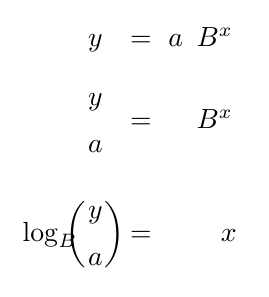
\begin{tikzpicture}[x=1em,y=-1em]
\node[anchor=base, inner sep=0pt] at (6.76,2.72) {$\pFourCell{1.92}{B^{{\scriptstyle x}}}$};
\node[anchor=base, inner sep=0pt] at (2.45,2.72) {$\pFourCell{0.9}{y}$};
\node[anchor=base, inner sep=0pt] at (4.09,2.72) {$\pFourCell{1.62}{=}$};
\node[anchor=base, inner sep=0pt] at (5.35,2.72) {$\pFourCell{0.9}{a}$};
\node[anchor=base, inner sep=0pt] at (6.76,5.67) {$\pFourCell{1.92}{B^{{\scriptstyle x}}}$};
\node[anchor=base, inner sep=0pt] at (2.45,5.67) {$\pFourFraction{0.9em}{\pFourCell{0.9}{y}}{\pFourCell{0.9}{a}}$};
\node[anchor=base, inner sep=0pt] at (4.09,5.67) {$\pFourCell{1.62}{=}$};
\node[anchor=base, inner sep=0pt] at (2.45,9.75) {$\pFourFraction{0.9em}{\pFourCell{0.9}{y}}{\pFourCell{0.9}{a}}$};
\node[anchor=base, inner sep=0pt] at (0.81,9.75) {$\pFourCell{1.62}{\pFourCell{1.62}{\log_{B}}}$};
\node[anchor=base, inner sep=0pt] at (1.81,9.75) {$\pFourCell{0.38}{\left(\rule[-1em]{0pt}{1.96em}\right.}$};
\node[anchor=base, inner sep=0pt] at (3.09,9.75) {$\pFourCell{0.38}{\left.\rule[-1em]{0pt}{1.96em}\right)}$};
\node[anchor=base, inner sep=0pt] at (4.09,9.75) {$\pFourCell{1.62}{=}$};
\node[anchor=base, inner sep=0pt] at (7.27,9.75) {$\pFourCell{0.9}{x}$};
\end{tikzpicture}
\end{center}


\newpage
\section*{Spaltentreue LaTeX-Ausgabe mit Spaltengrenzen}
\vspace{6mm}
\begin{center}
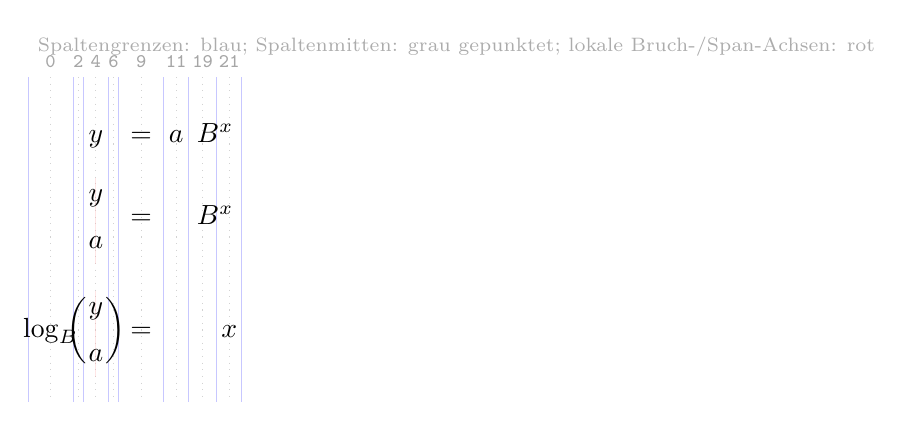
\begin{tikzpicture}[x=1em,y=-1em]
\node[font={\scriptsize}, text=gray!65, anchor=west] at (0,-0.75) {Spaltengrenzen: blau; Spaltenmitten: grau gepunktet; lokale Bruch-/Span-Achsen: rot};
\draw[blue!22, line width=0.28pt] (0,0.35) -- (0,12.1);
\draw[blue!22, line width=0.28pt] (1.62,0.35) -- (1.62,12.1);
\draw[blue!22, line width=0.28pt] (2,0.35) -- (2,12.1);
\draw[blue!22, line width=0.28pt] (2.9,0.35) -- (2.9,12.1);
\draw[blue!22, line width=0.28pt] (3.28,0.35) -- (3.28,12.1);
\draw[blue!22, line width=0.28pt] (4.9,0.35) -- (4.9,12.1);
\draw[blue!22, line width=0.28pt] (5.8,0.35) -- (5.8,12.1);
\draw[blue!22, line width=0.28pt] (6.82,0.35) -- (6.82,12.1);
\draw[blue!22, line width=0.28pt] (7.72,0.35) -- (7.72,12.1);
\draw[gray!35, dotted] (0.81,0.35) -- (0.81,12.1);
\node[font={\ttfamily\scriptsize}, text=gray!70, anchor=base] at (0.81,0) {0};
\draw[gray!35, dotted] (1.81,0.35) -- (1.81,12.1);
\node[font={\ttfamily\scriptsize}, text=gray!70, anchor=base] at (1.81,0) {2};
\draw[gray!35, dotted] (2.45,0.35) -- (2.45,12.1);
\node[font={\ttfamily\scriptsize}, text=gray!70, anchor=base] at (2.45,0) {4};
\draw[gray!35, dotted] (3.09,0.35) -- (3.09,12.1);
\node[font={\ttfamily\scriptsize}, text=gray!70, anchor=base] at (3.09,0) {6};
\draw[gray!35, dotted] (4.09,0.35) -- (4.09,12.1);
\node[font={\ttfamily\scriptsize}, text=gray!70, anchor=base] at (4.09,0) {9};
\draw[gray!35, dotted] (5.35,0.35) -- (5.35,12.1);
\node[font={\ttfamily\scriptsize}, text=gray!70, anchor=base] at (5.35,0) {11};
\draw[gray!35, dotted] (6.31,0.35) -- (6.31,12.1);
\node[font={\ttfamily\scriptsize}, text=gray!70, anchor=base] at (6.31,0) {19};
\draw[gray!35, dotted] (7.27,0.35) -- (7.27,12.1);
\node[font={\ttfamily\scriptsize}, text=gray!70, anchor=base] at (7.27,0) {21};
\node[anchor=base, inner sep=0pt] at (6.76,2.72) {$\pFourCell{1.92}{B^{{\scriptstyle x}}}$};
\node[anchor=base, inner sep=0pt] at (2.45,2.72) {$\pFourCell{0.9}{y}$};
\node[anchor=base, inner sep=0pt] at (4.09,2.72) {$\pFourCell{1.62}{=}$};
\node[anchor=base, inner sep=0pt] at (5.35,2.72) {$\pFourCell{0.9}{a}$};
\node[anchor=base, inner sep=0pt] at (6.76,5.67) {$\pFourCell{1.92}{B^{{\scriptstyle x}}}$};
\draw[red!30, opacity=0.32, line width=0.35pt] (2.45,3.99) -- (2.45,7.12);
\node[anchor=base, inner sep=0pt] at (2.45,5.67) {$\pFourFraction{0.9em}{\pFourCell{0.9}{y}}{\pFourCell{0.9}{a}}$};
\node[anchor=base, inner sep=0pt] at (4.09,5.67) {$\pFourCell{1.62}{=}$};
\draw[red!30, opacity=0.32, line width=0.35pt] (2.45,8.07) -- (2.45,11.2);
\node[anchor=base, inner sep=0pt] at (2.45,9.75) {$\pFourFraction{0.9em}{\pFourCell{0.9}{y}}{\pFourCell{0.9}{a}}$};
\node[anchor=base, inner sep=0pt] at (0.81,9.75) {$\pFourCell{1.62}{\pFourCell{1.62}{\log_{B}}}$};
\node[anchor=base, inner sep=0pt] at (1.81,9.75) {$\pFourCell{0.38}{\left(\rule[-1em]{0pt}{1.96em}\right.}$};
\node[anchor=base, inner sep=0pt] at (3.09,9.75) {$\pFourCell{0.38}{\left.\rule[-1em]{0pt}{1.96em}\right)}$};
\node[anchor=base, inner sep=0pt] at (4.09,9.75) {$\pFourCell{1.62}{=}$};
\node[anchor=base, inner sep=0pt] at (7.27,9.75) {$\pFourCell{0.9}{x}$};
\end{tikzpicture}
\end{center}
\end{document}
